\documentclass{article}
             \usepackage{graphicx}
             \usepackage[colorlinks]{hyperref} 
             \usepackage{url}
             \usepackage{float}
             \usepackage[landscape]{geometry} 
\title{Report generated by Pmetrics package for R on 10 Mar 2020 at 15:37 } 
\date{}
              \begin{document}
              \maketitle 
Laboratory of Applied Pharmacokinetics $\cdot$ 4650 Sunset Blvd. MS\#51, Los Angeles, CA 90027 $\cdot$ (323) 361-5046 $\cdot$ \href{http://www.lapk.org}{www.lapk.org} 
\hypertarget{tableofcontents}{}
        \tableofcontents
        \newpage 
\section{Summary} \hyperlink{tableofcontents}{Back to Contents} $\cdot$ \hyperlink{cycleinfo}{Next Section}\newline
 \newline 
Engine: IT2B\newline 
Output file: /Users/Neely/LAPK/Development/Pmetrics/data-raw/Runs/2/outputs/IT\_RF0001.TXT\newline 
Random parameters:Ka, Ke, V, Tlag1\newline 
There were no random fixed parameters. \newline 
There were no constant fixed parameters. \newline 
Number of analyzed subjects:  20 \newline 
Number of output equations:  1 \newline 
Number of cycles:  20     - The run converged. \newline 
Additional covariates:  WT, AFRICA, AGE, GENDER, HEIGHT \newline 
 \newline 
\newpage
            \hypertarget{cycleinfo}{}
            
            \section{Cycle information} \  
 $\cdot$ \hyperlink{tableofcontents}{Back to Contents} $\cdot$ \hyperlink{mppd}{Next Section} \newline 
\begin{figure}[H] 
            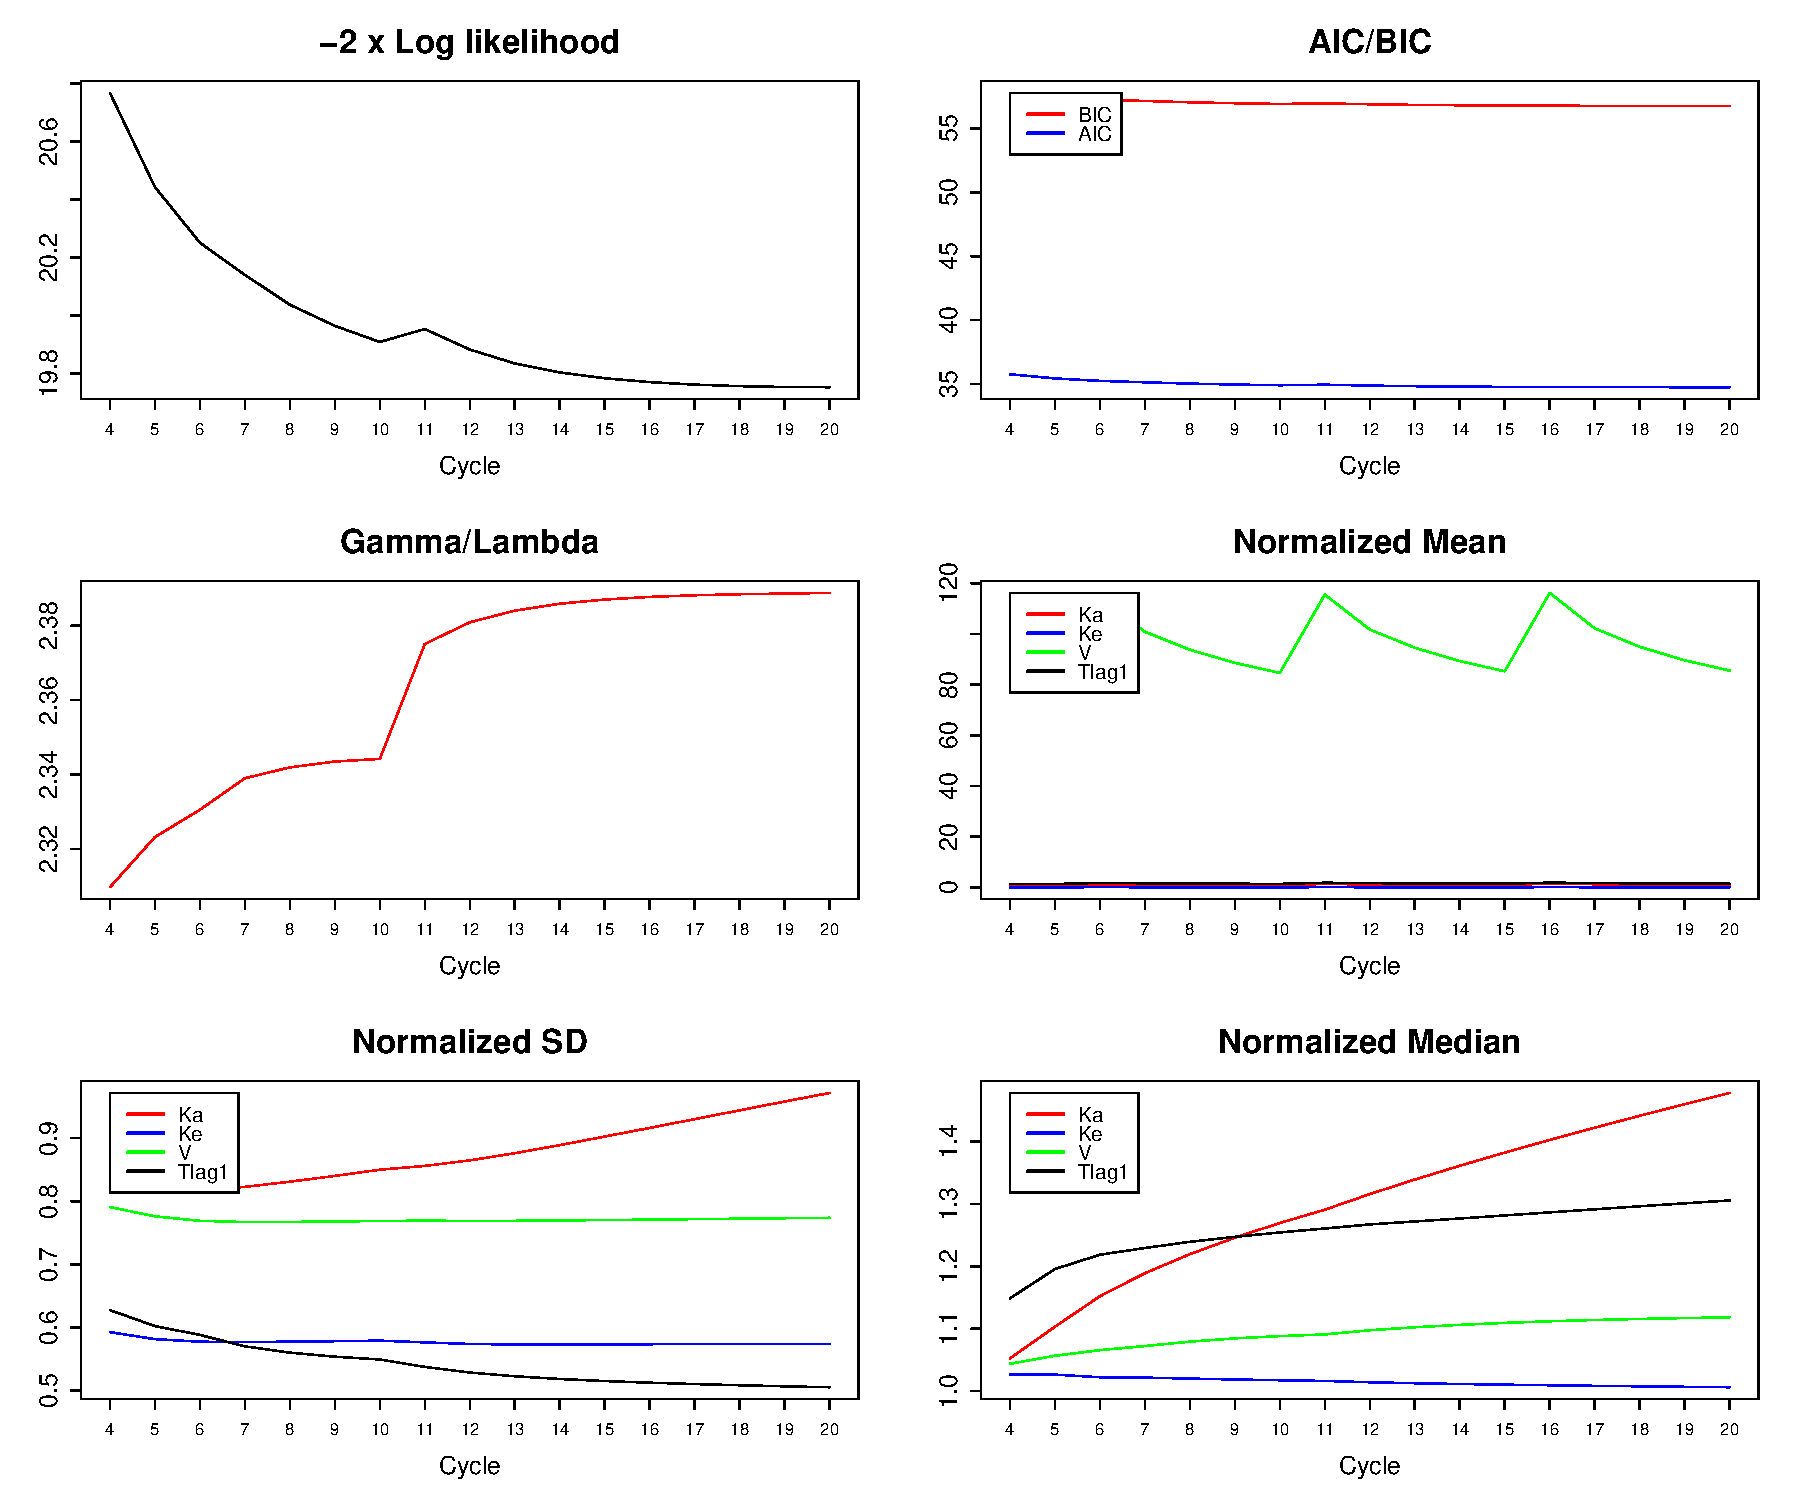
\includegraphics[height=4.99in,width=7in]{cycle.pdf}
            \end{figure} 
\hypertarget{mppd}{}
          \section{Marginal population parameter distributions} 
 $\cdot$ \hyperlink{tableofcontents}{Back to Contents} $\cdot$ \hyperlink{suppoint}{Next Section} \newline
           
\begin{figure}[H] 
          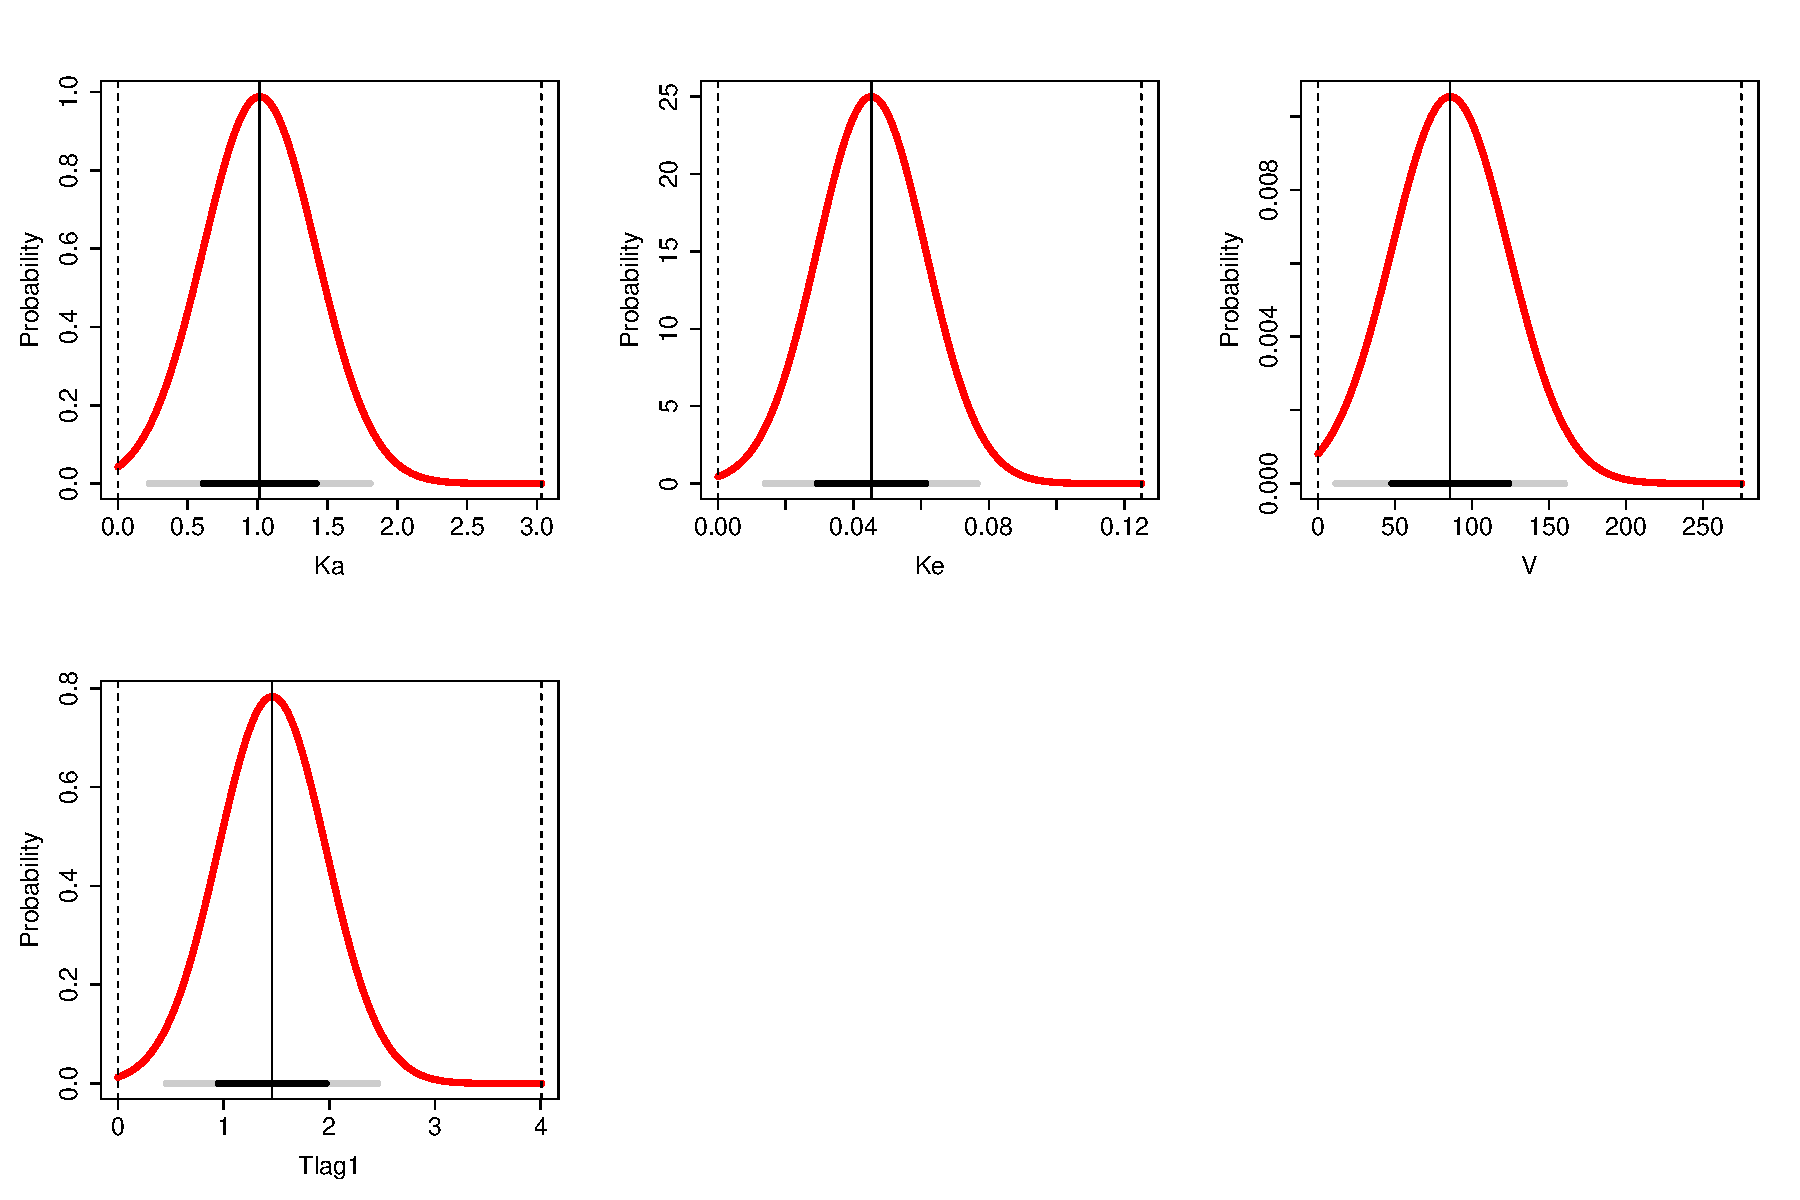
\includegraphics[height=4.5in,width=8in]{final.pdf}
          \end{figure} 
              
          \hypertarget{ppe}{}
          
          \section{Population parameter estimate summary statistics} 
 \hyperlink{tableofcontents}{Back to Contents} $\cdot$ \hyperlink{covforppe}{Next Section} \newline
          \newline 
